\documentclass[a4paper, amsfonts, amssymb, amsmath, reprint, showkeys, nofootinbib, oneside]{revtex4-1}
\usepackage[english]{babel}
\usepackage[utf8]{inputenc}
\usepackage[colorinlistoftodos, color=green!40, prependcaption]{todonotes}
\usepackage{amsthm}
\usepackage{mathtools}
\usepackage{physics}
\usepackage{xcolor}
\usepackage{graphicx}
\usepackage[left=23mm,right=13mm,top=35mm,columnsep=15pt]{geometry} 
\usepackage{adjustbox}
\usepackage{placeins}
\usepackage[T1]{fontenc}
\usepackage{lipsum}
\usepackage{csquotes}
\usepackage[pdftex, pdftitle={Article}, pdfauthor={Author}]{hyperref} % For hyperlinks in the PDF
%\setlength{\marginparwidth}{2.5cm}
\bibliographystyle{apsrev4-1}
\usepackage{array}
\usepackage{longtable}
\usepackage{multirow}

\begin{document}
%\title{\textcolor{red}{Design strategies for the self-assembly of polyhedral shells using SAT-assembly}}
%\title{Design strategies for the self-assembly of polyhedral shells}
\title{SAT-assembly of polyhedral shells}

\author{Diogo E. P. Pinto$^1$, Petr $\check{\text{S}}$ulc$^2$, Francesco Sciortino$^1$ and John Russo$^1$}
    \email[Correspondence email address: ]{john.russo@uniroma1.it}% Your name
    \affiliation{$^1$Dipartimento di Fisica, Sapienza Universit\`{a} di Roma, P.le Aldo Moro 5, 00185 Rome, Italy}
    \affiliation{$^2$School of Molecular Sciences and Center for Molecular Design and Biomimetics, The Biodesign Institute, Arizona State University, 1001 South McAllister Avenue, Tempe, Arizona 85281, USA}

\date{\today} % Leave empty to omit a date

\begin{abstract}
The control over the self-assembly of complex structures is a long-standing challenge of material science, especially at the colloidal scale, as the desired assembly pathway is often kinetically derailed by the formation of amorphous aggregates. Here we investigate in detail the problem of the self-assembly of
%the
three Archimedean shells,
%that can be assembled from five-coordinated unit, 
i.e. the icosahedron, the snub cube, and the snub dodecahedron. We use Patchy Particles with five interaction sites (or patches) as our model for the building blocks, and recast the assembly problem as a satisfiability problem (SAT) for the patch interactions. This allows us to find effective designs for all targets, and to selectively suppress unwanted structures.
By tuning the geometrical arrangement and the specific interactions of the patches, we find 
that lowering the symmetry of the building blocks is an effective way to reduce the number of competing structures, which in turn can considerably increase the yield of the target structure. We also consider the concentration dependence of our assemblies as a way to externally control which target structure is formed. These results cement SAT-assembly as an invaluable tool to solve inverse design problems.
\end{abstract}

\maketitle

\section{Introduction}

%The assembly of complex structures has been a longstanding challenge of material science \cite{Bishop2022}.
Self-assembly encompasses a large array of phenomena through which materials are formed using simple microscopic building blocks \cite{Whitelam2015}. In Nature, many striking examples of self-assembly are found, from virus capsids to lipid bilayers~\cite{Whitesides2002, Parnell2015, Teyssier2015}, but assembling new synthetic materials has proved to be very challenging. Successful examples of artificial self-assembly include three-dimensional crystals and polyhedral shells \cite{Dziomkina2005, Glotzer2007, Kim2011, LaCour2022,  McGorty2010, Mu2022, Nykypanchuk2008, Sacanna2011, Wang2012, Wang2015, Joshi2016,Bishop2022,Reguera2019, McMullen2022}. One of the main difficulties resides in how to optimize the geometrical properties or interactions between the building blocks without leading to kinetically arrested configurations~\cite{Frenkel2011, Lash2015, Blaaderen2006, Meulen2015}.

Here we focus on the self-assembly of finite-size structures and in particular on specific polyhedral shells. From an application standpoint, the potential of closed shells to act as a drug delivery system has been a widely researched topic, where a given drug is encapsulated within a closed shell and then driven to a specific diseased area where the drug is locally released such that the least amount of non diseased tissue is affected \cite{Huang2007, Uchida2007}. For this, the shell needs to close around a specific reagent and then open when external conditions are met. Recently, there have been suitable experimental realizations, for example, using DNA-origami, where selective interactions can be introduced to mimic patchy particles \cite{Mosayebi2017, Lee2022, Jun2021, Rothemund2006}.

When focusing on finite-size shells additional challenges arise compared to the ones encountered in the self-assembly of crystal structures. Firstly, the self-assembly occurs exclusively from the gas phase, which rules out the possibility to use (critical point induced) density fluctuations to accelerate the rate of aggregation, as frequently done in the case of crystals. On the contrary, the formation of finite-size aggregates stabilizes the gas phase to high densities with respect to the liquid phase, possibly introducing a density dependence of the aggregation pathway. Secondly, the small size of the aggregates, compared to the infinitely repeating units of a crystal, can stabilize kinetic straps, i.e. structures whose free-energy is not as low as the one of the target structure, but that require an exceedingly long waiting time to break. Lastly, the formation of finite-size aggregates is a continuous process, and is not accompanied by a phase transition as in crystals. The absence of a critical-size of formation (i.e. the critical nucleus) means that it is not sufficient to suppress a handful of competing structures at one length-scale, but that the assembly process has to proceed without defects at every stage. This problem is reflected in the difficulty of perfectly closing large-size aggregates, such as capsids~\cite{Mosayebi2017}.

Here we show how to successfully tackle these challenges by transforming the self-assembly problem into a satisfiability problem. This technique, named \emph{SAT-assembly}, was recently introduced by some of us to successfully assemble challenging crystalline structures,
with an emphasis on structures that have photonic applications, such as the tetrastack~\cite{Romano2020a} and diamond cubic crystal~\textcolor{blue}{\cite{Romano2020a,Russo2022,rovigatti2022simple}}, or structures with a high number of atoms in the unit cells, such as clathrate crystals~\cite{Romano2020a}.
In this article we will demonstrate a successful application of the SAT-assembly framework to the assembly of complex polyhedral shells. We focus on the three polyhedra that can assemble from building blocks with a  coordination number of five, i.e. the icosahedron, the snub cube, and the snub dodecahedron.
As building blocks we use patchy particles, which are a model of hard spheres with attractive patches on its surface \cite{Bianchi2006, Romano2010, Rovigatti2018, Russo2021, Sciortino2009}. These represent a coarse-grained approach to describe multiple systems, e.g. colloids, proteins, polymers, etc \cite{Sacanna2011, Wang2012}.
By associating to each patch a color, we can translate the self-assembly problem into the problem of finding how patch colours should interact to form the target structure, while at the same time avoiding competing structures.
%If to each patch is associated a color, one can formulate a problem with boolean variables which translates into a particle design (patch colors of a given particle, color-color interactions, etc.).
%One can then create an array of constraints that enforce the topology of a given target structure onto these variables~\cite{Russo2022} and use a SAT solver~\cite{Een2005} to efficiently find a design which satisfies the constraints imposed.

In the manuscript we will first show that, except for the smallest structure (the icosahedron), these shells do not assemble correctly if only the geometrical information about the target structure is used. Instead we will introduce multi-colored designs, i.e. designs where more than one patch type is present. As the number of patch types increases, so does the complexity of the design, making SAT a mandatory tool. We will show that the yield of the different structures depends sensitively on the particular geometrical patch arrangement and number of colors used, but that the different results can be rationalized by looking at the symmetry of the designs: less symmetrical building blocks self-assemble with the highest yield in the target structures. In particular, \emph{chiral} designs, i.e. not having a mirror-plane symmetry, are found to be very effective building blocks regardless of the chirality of the target structure. We also explore the role of geometrical frustration, where the angle between the patches does not match the angle between the particles in the target structure, to create designs where the target structure depends on external conditions (in our case the concentration of building blocks). Lastly, we emphasize how SAT is crucial to assemble a given structure while excluding competing ones. We find that mutual exclusion requires complex designs, with multiple patch colours and particle species (different patch colour arrangement in different particles), which lead to higher yields and assemblies that are more robust to geometrical frustrations.
%We will also consider the thermodynamic properties of the assembly process showing that our designs retain ideal behaviour up to very high densities, which explains the weak density dependence of the assembly yield. We conclude with a discussion and an outlook.

%To tackle these challenges, we explore the inverse design of finite-size structure via a novel technique, named SAT-assembly\cite{Romano2020a,Russo2022}. By describing the assembly as a constraint satisfiability problem (SAT), one is able to apply general tools to target the desired structures and exclude competing ones. One of its most successful applications is found in the design of patchy particles, where the building blocks are hard spheres with attractive patches on its surface \cite{Bianchi2006, Romano2010, Rovigatti2018, Russo2021, Sciortino2009}. These represent a coarse-grained approach to describe multiple systems, e.g. colloids, proteins, polymers, etc \cite{Sacanna2011, Wang2012}. If to each patch is associated a color, one can formulate a problem with boolean variables which translates into a particle design (patch colors of a given particle, color-color interactions, etc.). One can then create an array of constraints that enforce the topology of a given target structure onto these variables~\cite{Russo2022} and use a SAT solver~\cite{Een2005} to efficiently find a design which satisfies the constraints imposed.
%Another key advantage of SAT-assembly is that it doesn't require geometrical intuition on the target structure~\textcolor{blue}{\cite{rapaport2004self}}.


%So far, SAT-assembly has been used to study the assembly of complex crystals, with an emphasis on structures that have photonic applications, such as the tetrastack~\cite{Romano2020a} and diamond cubic crystal~\textcolor{blue}{\cite{Romano2020a,Russo2022,rovigatti2022simple}}, or structures with a high number of atoms in the unit cells, such as clathrate crystals~\cite{Romano2020a}. In this article we will first demonstrate a successful application of the SAT-assembly framework to the assembly of complex polyhedral shells. We focus on the three polyhedra that can assemble from building blocks with a  coordination number of five, i.e. the icosahedron, the snub cube, and the snub dodecahedron. Except for the smallest structure (the icosahedron), these shells do not assemble correctly if only the correct geometry of the patches is used, but instead require the introduction of multi-colored designs, i.e. designs where more than one patch type is present. As the number of patch types increases, so does the complexity of the design, making SAT a mandatory tool. We will show that the yield of the different structures depends sensitively on the particular geometrical patch arrangement and number of colors used, but that the different results can be rationalized by looking at the symmetry of the designs: less symmetrical building blocks self-assemble with the highest yield in the target structures. In particular, \emph{chiral} designs, i.e. not having a mirror-plane symmetry, are found to be very effective building blocks regardless of the chirality of the target structure. We also explore the role of geometrical frustration, where the angle between the patches does not match the angle between the particles in the target structure, to create designs where the target structure depends on external conditions (in our case the concentration of building blocks). Lastly, we emphasize how SAT is crucial to assemble a given structure while excluding competing ones. We find that mutual exclusion requires complex designs, with multiple patch colours and particle species (different patch colour arrangement in different particles), which lead to higher yields and assemblies that are more robust to geometrical frustrations. We will also consider the thermodynamic properties of the assembly process showing that our designs retain ideal behaviour up to very high densities, which explains the weak density dependence of the assembly yield. We conclude with a discussion and an outlook.





\section{Models}


\begin{figure}[t]
	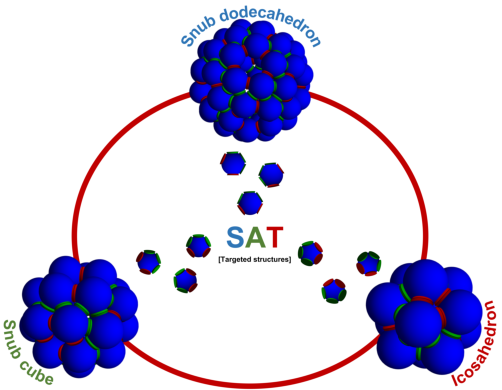
\includegraphics{fig1.pdf}
	\caption{\label{SAT} Schematic representation of the structures explored. A particle with valence 5 is used to assemble the different polyhedron shells. A solution calculated with SAT is used for the patchy particle design which satisfies all three structures. It contains only one particle specie (blue) and two patch colors (green and red). The green patches only interact with green while the red only interact with red.}
\end{figure}

We consider a system composed of $N$ patchy particles in a cubic box of length $L$. The particles are characterized by a hard core of radius $\sigma$ with five patches on its surface located on one side of the particle forming a star-like shape with mirror symmetry along one of the patches (as seen in the center of Fig.~\ref{SAT}).
We follow the same SAT formulation as the one in Ref.~\cite{Russo2022}. We consider that each patch can have a given color between $1\leq x_c\leq N_c$, where $N_c$ is the total number of colors. These colors can be distributed onto the patches in specific arrangements, each unique sequence can be considered a particle specie, thus $1\leq x_p\leq N_p$, where $N_p$ is the total number of species. SAT is then used to find if a given combination of $N_p$ and $N_c$ can satisfy a given polyhedral shell, e.g. if it satisfies all the topological constraints, and a solution/design is calculated which can be used to prepare the composition of the system. In the \emph{Supplemental Material} we go into more detail on the different constraints (clauses) used in SAT.
We study the self-assembly outcome of our designs via Monte Carlo simulations using aggregation-biased moves and using the Kern-Frenkel portential~\cite{Kern2003} to describe the interaction between patches (See Methods).

Our self-assembly problem is represented schematically in Fig.~\ref{SAT}. Starting with patchy particles of valence five we wish to selectively assemble three Archimedean polyhedral shells: the 12-particle \emph{icosahedron}, the 24-particle \emph{snub cube}, and the 60-particle \emph{snub dodecahedron}. When perfectly arranged, these structures differ for the in-plane angle that patches 4 and 5 make with the center of the particle, which we call $\gamma$ in Fig.~\ref{SAT}: this is $\gamma=60^\circ$ for the icosahedron, $\gamma=90^\circ$ for the snub cube, and  $\gamma=108^\circ$ for the snub dodecahedron. We consider two geometrical control parameters: the angular width of the patch interaction, $\cos\theta_\text{max}$, and the in-plane angle $\gamma$. On top of the geometrical parameters, we also vary the patch colouring, i.e. we distribute $N_c$ colours among the patches and then use the SAT-assembly algorithm to derive an interaction table among the colours such that all bonds in the target structure(s) are satisfied. Finally we also vary the temperature and density conditions of the assembly to study the phase behaviour of our designs.


\section{Geometrical designs}


\begin{figure}[t]
	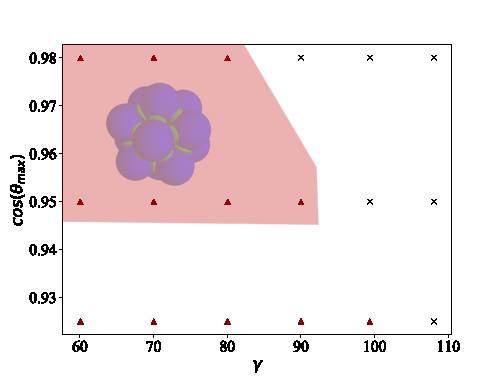
\includegraphics{fig2.pdf}
	\caption{\label{N1c1} Most probable structure formed for different in-plane angles, $\gamma$, between $\textbf{p}_4$ and $\textbf{p}_5$ in Eq.~\ref{patch} and for different patch width, $\cos\theta_{max}$, in Eq.~\ref{KF}. The triangles inside the red region represent parameters where the most probable polyhedron shell from the ones in Fig.~\ref{SAT} is the icosahedron. Black crosses represent systems where open/incomplete clusters are more probable. The gray stars represent systems where clusters are able to close but none correspond to the ones in Fig.~\ref{SAT}. We find that for the most trivial solution only the icosahedron is able to form.}
\end{figure}


To consider geometric effects only, we fix one patch color (i.e. each patch can interact with all others), and explore different values of the patch width, $\cos\theta_{max}$ (in Eq.~\ref{KF}, where we drop $\alpha$ and $\beta$ for simplicity) as well as different geometries of the patches by changing the in-plane angle $\gamma$ created by $\textbf{p}_4$ and $\textbf{p}_5$ in Eq.~\ref{patch}. The former allows for more flexibility of the bonds due to larger patch widths. The latter improves our ability to target the different structures proposed in Fig.~\ref{SAT} by more easily satisfying their geometry.
%For example, if the in plane angle between these vectors is close to $90$ degrees it is easier to form the squares in the snub cube.

Figure \ref{N1c1} summarizes the results, showing the most probable closed structure assembled for each value of $\cos\theta_{max}$ and $\gamma$ considered. As represented by the triangle symbols (and the shaded area), we find that only the icosahedron is able to form for the range of parameters explored, while the snub cube and snub dodecahedron fail to assemble even when the geometry of the particles is the ideal one ($\gamma=90^\circ$ for the snub cube, and  $\gamma=108^\circ$ for the snub dodecahedron).

We classify the state points where no target structure is formed into two groups. The gray stars correspond to irregular aggregates, thus clusters more akin to micelles, that close without defects but don't have a regular shape. If no closed structure is formed, we use black crosses to classify the state point, the ones where particles form bonds but they do not close, thus forming an open shell.
%They are irregular in the sense that they do not correspond to any specific polyhedron.

These results confirm the well-known fact that self-assembly designs cannot generally rely only on the geometrical properties of the building units alone. In our case, only the smallest target structure, the icosahedron, is successfully assembled. The assembly is limited at large values of $\gamma\sim 90^\circ$, above which the geometry of the building unit is not compatible with bond formation in the target structure and only incomplete structure are formed. As expected, the $\gamma$ range increases for increasing patch width (lowering $\cos\theta_{max}$). But crucially the assembly is also limited at large patch widths, $\cos\theta_{max}>0.95$, below which mostly irregular structures are observed. With large patch widths there are multiple ways for a shell to close onto itself, and this degeneracy entropically stabilizes irregular structures over the more ordered polyhedral shells. We note that although icosahedron structures are still observed for large patch widths, $\cos\theta_{max}<0.95$, a lot fewer are completely assembled (less than 5\%). In the following we will show that this degeneracy in allowed structures can be overcome by reducing the symmetry of the building blocks with patch colouring.


%We find that only the icosahedron is able to form for the range of parameters explored. Furthermore, increasing patch width (lowering $\cos\theta_{max}$), thus increasing bond flexibility hinders the assembly of these structures. We can conclude that it is not sufficient for a particle and patch design to satisfy the targeted structure for it to assemble.

\section{SAT designs}

\subsection{Patch colouring}


\begin{figure}[t]
	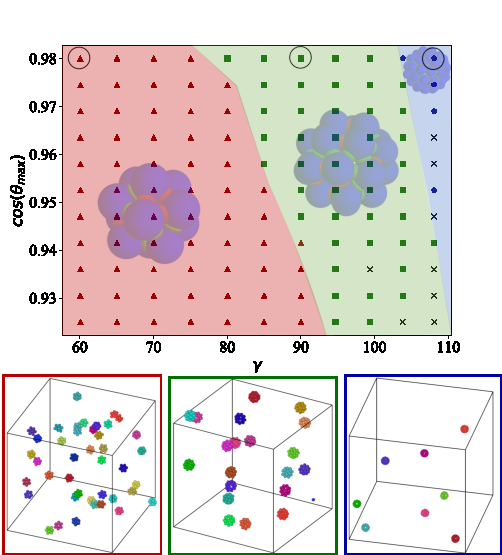
\includegraphics{fig3.pdf}
	\caption{\label{N1c2} Most probable structure formed for different in-plane angles, $\gamma$, between $\textbf{p}_4$ and $\textbf{p}_5$ in Eq.~\ref{patch} and for different patch width, $\cos\theta_{max}$, in Eq.~\ref{KF}. The triangles inside the red region represent parameters where the most probable structure from the ones in Fig.~\ref{SAT} is the icosahedron. The squares inside the green region represent parameters where the most probable structure from the ones in Fig.~\ref{SAT} is the snubcube. The pentagons inside the blue region represent parameters where the most probable structure from the ones in Fig.~\ref{SAT} is the snub dodecahedron. Black crosses represent systems where open/incomplete clusters are more probable. The gray stars represent systems where clusters are able to close but none correspond to the ones in Fig.~\ref{SAT}. On the bottom are typical configurations from the parameters that are encircled in the plot. They were imaged with OVITO and the colors represent different clusters. The design used was of one specie and two colors, where all interactions are self-similar (red with red and green with green).}
\end{figure}


%We now consider a non trivial design but with minimal colors and species.
In contrast to the previous section, we now break the interaction symmetry, and introduce patch colours.
We start by considering a solution that satisfies all three polyhedral structures with only one particle specie and two patch colors. We employ SAT to satisfy such constraints and extract the proper patch ordering and interactions.
The solution is represented schematically as the first entry in the table in Fig.~\ref{Yield}, and the interactions are allowed only among patches of the same group (green with green, red with red): $1$, $2$ and $3$ (green) on one side, and $4$ and $5$ (red) on the other.

In Fig.~\ref{N1c2} we display the results for this design, showing which structures are formed depending on the geometrical parameters $\cos\theta_{max}$ and $\gamma$. Comparing these results with Fig.~\ref{N1c1}, we observe that all three polyhedral shells can be assembled within the parameters explored. Differently from before, the structures form at all values of $\cos\theta_{max}$ considered, and the dominant structure is controlled primarily by the angle $\gamma$, with the stability of each structure approximately centered around its optimal angle. As observed before, structures with fewer particles are favored when the patch width increases: this is an entropic effect, as fully formed shells behave as an ideal gas of clusters, whose entropy increases with number density of clusters. Snapshots of the gas of icosahedral, snub cube, and snub dodecahedron are shown in the lower panels of Fig.~\ref{N1c2}.

Already from the results of Fig.~\ref{N1c2} we can assert that even the introduction of minimal patch colouring significantly improves the self-assembly process. In the next section we will look in detail the effects of different colouring patterns on the yield of self-assembly.

%Examples of successful assembly simulations are displayed in the snapshots of Fig.~\ref{N1c2}. Thus, one can significantly improve on the trivial solution by using SAT as a design tool to assemble finite-size shells, even with minimal colors and species. These results also suggest that as patch width increases, structures with fewer particles are favored. Since the icosahedron requires less particles to form, the patch width compensates for the change in geometry (in plane angle of the patches).

\subsection{Patch patterning}

The table in Fig.~\ref{Yield} contains seven different patch patterning designs, varying the number of colours and the interaction among them. As the number of colours increases, so does the complexity of the design. As such, SAT becomes essential to extract the ordering and interactions such that all structures are possible. The name of the design expresses the number of colours used and, in parenthesis, different patterning choices: for example, $C4(1)$ and $C4(2)$ are two different designs with 4 colours. Each design is compatible with all three target structures, and we test them for three geometrical arrangements of the patches, differing for their angle $\gamma\in [60^\circ, 90^\circ, 108^\circ]$. It is important to note that for $\gamma=60^\circ$ all patches are geometrically indistinguishable, i.e. the angle between any two adjacent patches and the center of the particle is the same $60^\circ$. For the other values of $\gamma$, instead, the only geometric symmetry of the particles is a vertical mirror plane as shown in Fig.~\ref{SAT}. This last symmetry can be broken by introducing patch colouring. By colour-symmetry we refer to the presence of symmetry elements (in our case the vertical mirror plane) which bring a specific design into self-coincidence after (eventually) exchanging the identity of the colours. For example, let's consider the design C3(1) in Fig.~\ref{Yield}: patches $(1,2,3)$ are green, patch $4$ is red, and patch $5$ is orange. The design has colour symmetry because after reflecting all patches through the vertical mirror plane, and after the following colour exchange $(\text{red}\leftrightarrow\text{orange})$, the design remains the same.
%whose effect is to exchange the positions of interacting patches.
In the following we will investigate how colour-symmetry correlates with self-assembly yield.

\begin{figure*}[t]
	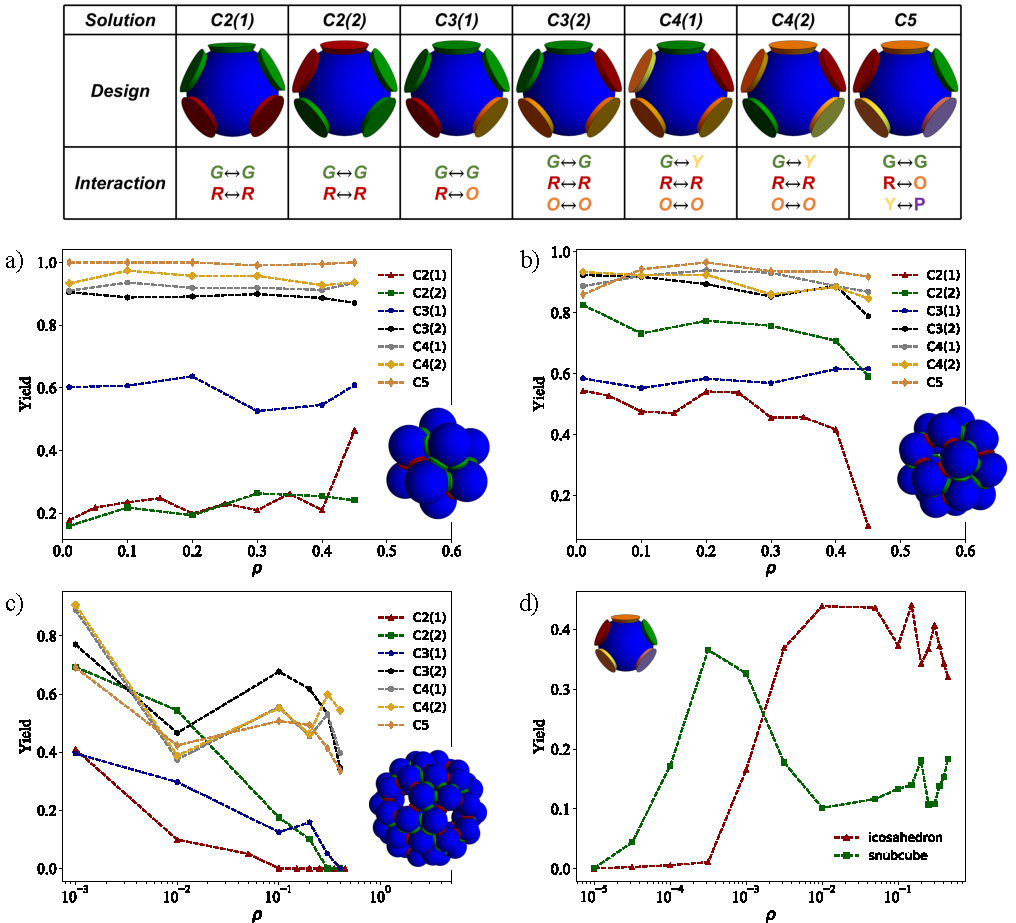
\includegraphics{fig4.pdf}
	\caption{\label{Yield} Average yield of the icosahedron, snub cube and snub dodecahedron (in Fig.~\ref{SAT}) as a function of the density of patchy particles (a, b and c plots respectively). These results were calculated with $\cos\theta_{max}=0.98$ and the in-plane angle, $\gamma$, was chosen to be the best for each structure. Thus, the icosahedron curve was calculated with $\gamma=60^\circ$, the snub cube with $\gamma=90^\circ$ and the snub dodecahedron with $\gamma=90^\circ$. Different solutions were explored which are summarized in the table above the plots, where the respective designs and interactions are shown. d) shows the average yield as a function of density for a design of five colors. Here, both curves were measured for the same system with $\gamma=85.45^\circ$ and $\cos\theta_{max}=0.947$. All results shown in this figure were calculated at $T=0.097$.}
\end{figure*}

%shows the different yields of the polyhedron shells using the most optimized in plane angle for each ($60$ degrees for the icosahedron, $90$ degrees for the snub cube and $108$ degrees for the snub dodecahedron).
In Fig.~\ref{Yield} we plot the density dependence of the yield for all designs and for $\gamma=60^\circ$ (panel a), $\gamma=90^\circ$ (panel b), and $\gamma=108^\circ$ (panel c).
We define the yield as the probability of finding a cluster corresponding to a specific structure. We count single particles as a cluster of size one, and any bonded particles as clusters of size two or above, depending on the number of particles bonded.
We stress the fact that we measure the equilibrium yield, i.e. the yield after long waiting times, as our AVB biased moves allow us to rapidly form bonds regardless of the system density.

We can summarize the results of Fig.~\ref{Yield} with the following observations.


\noindent
\emph{1. Increasing the number of colours increases the yield.} Regardless of the target structure, and with few exceptions detailed below, the yield increases with the number of colours used. The increase is more significant for the first few colours added, while the yield's gain is more modest when the maximum number of colours is reached.
%At five colors the yield of the icosahedron and snub cube structures is close to maximum.
This is due to the fact that the probability of creating a wrong bound decreases with increasing number of colors. For example, in the C2(1) design, the top patches can form three possible connections, and thus the probability that the top three green patches form a correct bond is one third, while for the two red bottom ones is one half. The probability of correctly assembling the bonds to a central particle is then $(1/3)^3 (1/2)^2\sim 0.009$. As the number of colors increases so does the probability that a bond is formed correctly. So for the C5 design, there is only one possible bonding partner for each patch, and a particle can never form incorrect bonds.

\begin{figure*}[t]
	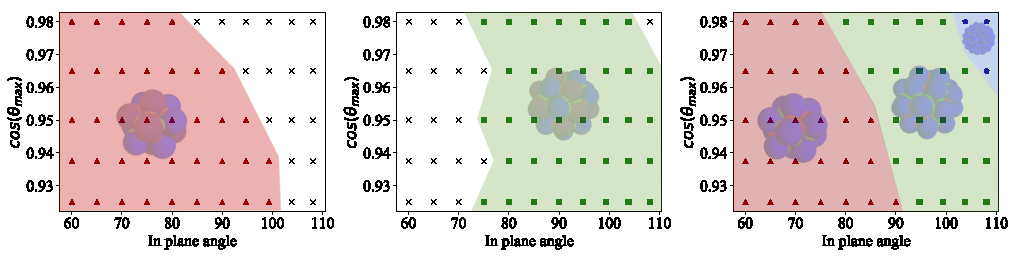
\includegraphics{fig6.pdf}
	\caption{\label{Sol} Most probable structure formed for different in-plane angles, $\gamma$, between $\textbf{p}_4$ and $\textbf{p}_5$ in Eq.~\ref{patch} and for different patch width, $\cos\theta_{max}$, in Eq.~\ref{KF}. Here, shell a) and b) are formed using a two species and five colors design which only satisfies each of the structures shown. On the left, the design only satisfies the icosahedron, in the middle, the snub cube. On the left, c), the design uses four species and twelve colours and only satisfies the snub dodecahedron.}
\end{figure*}

\noindent
\emph{2. Decreasing the symmetry of the building block increases the yield}. While for $\gamma=60^\circ$ the particles have a five-fold symmetry axis, altering the $\gamma$ angle orients the particles, making all patches distinguishable. The best example are designs C2(1) and C2(2), which are indistinguishable for $\gamma=60^\circ$, and whose yield increases significantly going from $\gamma=60^\circ$ to $\gamma=90^\circ$. Notice that the design C3(1) has a similar yield for $\gamma=60^\circ$ and $\gamma=90^\circ$. To understand this behaviour we need to introduce \emph{colour symmetry} below.

\noindent
\emph{3. Decreasing the colour symmetry of the patches increases the yield}. As mentioned before, all designs for $\gamma\neq 60^\circ$ have a single geometrical mirror plane, but patch colouring can maintain or break this symmetry. The designs that break the mirror-plane symmetry are \emph{chiral} designs: C2(2), C3(2), C4(1), C4(2), and C5. The designs that preserve the mirror-plane symmetry are \emph{achiral} designs: C2(1) and C3(1). Among the target structures, the icosahedron is an achiral assembly, while both the snub cube and the snub dodecahedron are chiral assemblies. We observe how in all cases chiral designs have higher yield compared to the achiral ones. This is true also for the icosahedron despite the lack of chirality in the target structure. For the snub cube and the snub dodecahedron we even observe that the yield of the chiral design C2(2) is higher than the achiral design C3(1) despite using less colours.


%seen in the table of Fig.~\ref{Yield}, all designs have the following colour simmetry: all patches go to a patch with a bond-compatible colour when reflected through the vertical mirror plane highlighted in Fig.~\ref{SAT}. Patch $2$, which is located on the mirror plane, is always self-interacting. This does not mean that all colouring schemes are equivalent, as the probability that a bond will be formed is influenced by how colours are distributed, even if the overall number of colours is the same. To understand this at a mean-field level, we consider the law of mass action, as written in Wertheim's theory~\textcolor{blue}{\cite{wertheim1984fluids,chapman1988phase,heras2011phase,teixeira2017phase}},
%which quantifies the probability for a patch $\alpha$ to be non-bonded, and which we denote by $X_{\alpha}$, where the index $\alpha$ runs over all patches, $\alpha\in[1,5]$

%\begin{equation}
%\label{prob}
%X_{\alpha}=\biggl[ 1+ \rho \sum_{\gamma=1}^5 \Upsilon_{\alpha,\beta} X_{\gamma} \Delta\biggr]^{-1}
%\end{equation}

%\noindent where $\Upsilon_{\alpha\beta}$ is unity when patches $\alpha$ and $\beta$ interact and zero otherwise, and $\Delta$ quantifies the strength of the interaction between interacting patches (see the Appendix for a detailed expression). Since all patches form independently (in Wertheim's theory), the probability $X_\alpha$ will be the same for all sets of interacting patches, and by denoting the number of patches with the same colour as $M_\alpha$ the equation becomes

%\begin{equation}
%X_{\alpha}=\biggl[ 1+ \rho M_\alpha X_{\alpha} \Delta\biggr]^{-1}
%\end{equation}

%Solving the equation above shows that the larger the number of patches with the same colour, $M_\alpha$, the smaller is $X_\alpha$, i.e. the larger is the probability for patch $\alpha$ to be bonded. These considerations allow us to divide the patches into different sets depending on the number of their bonding partners. We call these sets \emph{colour sets} and patches of the same set have the same bonding probability. Let's consider a few significant examples:
%\begin{itemize}
%\item As mentioned before, the C3(1) design has the same yield even after symmetry breaking (geometrically). But in this design patches $4$ and $5$ are each unique bonding partners, they cannot mis-bond, and so they break the rotational symmetry even for the case $\gamma=60^\circ$.
%\item The designs C2(1) and C2(2) have the same yield in the $\gamma=60^\circ$ particles, while C2(2) has a higher yield than C2(1) in the case $\gamma=90^\circ$. In the first case ($\gamma=60^\circ$), all patches are indistinguishable geometrically, and can be divided in two sets according to their colouring: patches $(1,2,3)$ and $(4,5)$ for design C2(1), and $(2,4,5)$ and $(1,3)$ for design C2(2). In this case the yield is the same. In the second case ($\gamma=90^\circ$), patches are divided in two groups geometrically, $(1,2,3)$ and $(4,5)$, which matches the colours sets of C2(1), but does not for C2(2). This difference between geometrical and coluring sets of patches is what makes the C2(2) design less symmetric and thus produces a higher yield.
%\item The same considerations of the previous example apply to designs C3(1) and C3(2). C3(1) has colour sets, $(1,2,3)$ and $(4,5)$, that overlap with the geometrical sets, while C3(2) breaks the symmetry with colour sets $(2)$, $(1,3)$, and $(4,5)$.
%\end{itemize}

\noindent
\emph{4. The yield has only a weak density dependence.} We observe that the yield of the different structures is constant with density. This means that clusters are fully formed in our thermodynamic conditions, and have ideal-gas behaviour. Only at high densities the yield starts decreasing, in correspondence with inter-cluster interactions and possibly a phase change to a liquid. Thermodynamics aspects of our assemblies will be examined in the last section. Interestingly, we also observe that large structures like the snub dodecahedron, which is composed of $60$ particles, is more easily assembled in very dilute systems where larger shells have more space to grow without influencing each other.


%We find that for this design, C2(1), the snub cube has the highest yield for all the densities explored except the last one. We also observe that large structures like the snub dodecahedron, which is composed of $60$ particles, is more easily assembled in very dilute systems where larger shells have more space to grow without influencing each other. The fact that the yield of the snub cube is higher than the icosahedron, even though its shell is larger, is probably due to the specific design used. In the case of the snub cube, the patchy particle geometry is already asymmetrical and the solution used helps enforce it in the assembly, thus the clusters that are not snub cubes are incomplete shells. On the other hand, the icosahedron patchy particle has some rigid body rotational symmetries. For example, if every patch has the same color, one can rotate each particle as a rigid body four times while still satisfying the same topology. In the design with two colors, this symmetry is lost. For the particles to satisfy the topology of the assembly, each needs to have specific orientation, thus losing the rigid body rotational symmetry given by the patch positions. This leads to many clusters which are formed with twelve particles (the number of particles in the icosahedron) but with one or two bonds missing for it to fully close. 

%In the same plots we show multiple other designs with only one specie, ranging from two colors to five. We find that, generally, the yield increases with the number of colors. At five colors the yield of the icosahedron and snub cube structures is close to maximum. This is due to the fact that the probability of creating a wrong bound decreases with increasing number of colors. For example, for the snub cube, there is only one specific bound that each patch can make in the final structure (since there is no rigid body rotational symmetry of the particles), but in the C2(1) case the top patches can form three possible connections. As such, the probability that the top three green patches form a correct bond is one third, while the two red bottom ones is one half. Thus, the probability of correctly assembling a particle is approximately $0.009$. As the number of colors increases so does the probability that a bond is formed correctly. For example, for the five colors there is only one possible bond formed for each patch (due to the interactions chosen) which is always the correct one. Thus, a particle can never form an incorrect bond. The only cases that do not follow this rule are the C2(1) and C2(2) designs. They share the same number of colors and are designed such that the probability of correct bonding is equal. Nonetheless, the average yield of the snub cube increases (from $\approx55\%$ to $\approx80\%$). We hypothesize that the design C2(2) creates a larger distinction between the patches than C2(1). In the case of the snub cube, the top three patches form the triangles seen in Fig.~\ref{SAT} while the two bottom patches form the square. In the design C2(1) the top three patches are indistinguishable, while in C2(2) its only a top one and the bottom two. Thus, in C2(2) the three top patches are now distinguishable by color while the bottom are by geometry. We hypothesize that this provides an easier pathway to assembly. The same is observed in the case of the snub dodecahedron, where now the bottom patches form pentagons. This is also supported by the fact that for the icosahedron, where all angles are the same, both designs have similar yields.

\noindent
\emph{5. Frustrated designs allow to target different structures depending on thermodynamic conditions.} In Fig.~\ref{Yield}\textit{d}  we plot the yield for a frustrated C5 design in which $\gamma=85.26^\circ$. The in-plane angle is close to the ideal angle for the assembly of the snub cube, which is indeed the most stable structure at low densities. But increasing the density we observe a switch to the smaller icosahedral shells. While the icosahedron has a much larger free energy of formation compared to the snub cube (due to the angle being unfavourable to the icosahedron), at high density this is compensated by the translational free energy (i.e. the ideal gas free energy), which is higher for the icosahedron (having a higher number density of clusters compared to the snub cube). The possibility to switch between different target structures as a function of external control parameters is a property of experimental interest.

Using the single specie designs we have measured several thermodynamic properties. For the C2(1) design, we show that the average potential energy has a non monotonic dependence with the density~\cite{Sciortino2009}. We also measured similar values for the critical miscelle concentration with three different designs, C2(1), C4(1), and C5, highlighting the weak dependence on patch colour. Using a simple mean-field model we are able to fit the temperature dependence of the critical miscelle concentration ~\cite{Kraft2012, Hatch2016}. See the \textit{Supplementary Material} for a more in-depth discussion.

\subsection{Structure selection}

In the previous examples, control over the target structure was obtained either geometrically (by changing the angles $\gamma$ and $\theta_\text{max}$ as in Fig.~\ref{N1c2}), or thermodynamically (by changing the density as in Fig.~\ref{Yield}d). Here we demonstrate that SAT-assembly allows to encode structure selection directly into the patch colouring. In particular we look for designs that satisfy only the icosahedron but not the snub cube and snub dodecahedron, and vice-versa. We find that the mutual exclusion of all three target structures requires at least two particle species for the snub cube and icosahedron, but four species for the snub dodecahedron. Here we show results with two species and five colours $N_c=5$ for the icosahedron and snub cube and four species and twelve colours $N_c=12$ for the snub dodecahedron, even if other solutions with different number of colours also exist. The results with our selected designs are shown in Fig.~\ref{Sol}. For the two species design we highlight that a mutually exclusive selection of the target structures can be achieved via non trivial patch colour ordering using SAT.



%Lastly, we focus on a more complex design with two species and five colors. In this case we force SAT to calculate a solution that only satisfies one of the structures of Fig.~\ref{SAT}. Figure \ref{Sol} shows the results with the corresponding design. Using SAT it is possible to generate solutions which exclude specific structures. Thus, one can, for example, calculate a solution that satisfies the topological constraints of the icosahedron but does not of the snub cube or snub dodecahedron. 
Comparison with the 1-specie solution (see Fig.~\ref{N1c2}) shows that suppression of the competing structure significantly enlarges the range of parameters where a certain shell is formed. Finally, the absence of competing structures also increases the yield to almost $100\%$ in some regions of the parameter space (not shown).

Incidentally, we note that targeting only the snub dodecahedron is complicated by the fact that all two species designs found by SAT are compatible with the formation of icosahedron or snub cube structures from only one of the two species, practically pre-emptying the formation of the target structure. As such, the number of species needs to increase in order to find a suitable design that satisfies the snub dodecahdron while completely excluding the others. We found that a four species design satisfies the constraint. Using SAT, one can calculate a solution for the snub dodecahedron and then check if it (or any of its subsets) also satisfies the other structures. If so, this solution is excluded and a new one is generated until all solutions are exhausted. Therefore, it is possible that designs with fewer species satisfy our constraints, but require significant computational resources to find using this method.

We note that the range of parameters where the snub dodecahedron is formed enlarges, but not as much as the icosahedron or the snub cube. In fact, the snub dodecahedron is not as robust to geometrical frustrations as the other structures. As $\gamma$ approaches $90^\circ$, snub cubes start forming due to geometrical incompatibilities, but given the colouring they never fully close. These almost complete structures require a large amount of time to break.

%while also we also increase its yield, since it is more rare to find competing structures. Both for the icosahedron and snub cube designs we observe the increase of the parameter ranges over more in plane angles as well as $\cos\theta_{max}$, meaning that they are more resilient to changes in the geometry of the patches and width of the interactions. On the other hand, the diagram of the snub dodecahedron does not change substantially when compared to Fig~\ref{N1c2}. In this case, although the two species and five colors solution only satisfies the snub dodecahedron, one of the species, by itself, is able to form the other competing shells. We hypothesize that this will always be the case for any design, since the topology of the snub dodecahedron is almost the same as the snub cube, in term of which bonds are formed between particles and their orientations. Only one particle is the exception which is necessary to close the snub dodecahedron and not the snub cube. Thus, in any design with more than one species that satisfies the snub dodecahedron, there might be a subset of those species that will always satisfy the snub cube as well. We have explored all solutions in the two species case, varying the number of colors from two to ten, and in all one of its subsets always satisfies other shells (icosahedron or snub cube). One could try to exhaust (by brute force) all possible species and color combinations but as species and colors increase so do the number of solutions (and its subsets) making this a very demanding task.

\section{Conclusions}

In this work we have explored design principles that can guide the formation of complex target structures, and applied them to regular polyhedral shells of valence five, i.e. the icosahedron, the snub cube, and the snub dodecahedron. In particular we have demonstrated that the target structure can be effectively encoded in simple patchy particle models by tuning simple geometrical parameters of the particle and/or the inter-particle interactions.

Choosing the correct inter-particle designs (i.e. patch colouring) is a complex optimization problem that we solve by encoding the bond topology in a set of satisfiability equations. This approach, named SAT-assembly, not only efficiently searches the space of possible designs for solutions which have the target structure as an energy minima, but also allows to explicitly enforce the non-satisfiability of competing structures as a way of avoiding the formation of kinetic aggregates.

Starting from solutions which target at the same time all the structure of interest, we have explored the effects of patch geometry, patch colouring, and patch patterning on the aggregate's yield. We find that the symmetry of the building blocks plays a key role in determining the yield of the final structure, with chiral designs consistently producing high yields for all structures considered. Introducing frustration by altering the patch geometry from the ideal one, is a promising strategy to produce designs with target structures that depend on external conditions.
%and highlight the  Breaking the geometric symmetries Less symmetric designs are less degenerate, i.e. they admit fewer incorrect bonding patterns, and allow for considerable gains in yield.  

%By exploring the space of two-species solutions


%In this work we have shown how to translate the self-assembly of finite-size structures using patchy particles into a SAT problem. Using patchy particles of valence five we explored different structures through Monte Carlo simulations and how to optimize the parameters to enhance self-assembly. We have proved that doing the most trivial design of patchy particles (one specie and one color) is worse than using SAT. While the most trivial design only yields one of the possible three shells, by slightly increasing the complexity of the design (adding one color) and allowing SAT to color the patches we find an overall improvement. The SAT design not only increases the probability of forming the finite size structures but allows us to explore different structures. Thus, we show that with these patchy particles one can form the icosahedron, snub cube or snub dodecahedron. We also show how these structures are affected by density, showing that larger structures are harder to assemble in higher densities and smaller ones, like the icosahedron, are favored due to their small size leading to an increase in yield.

We used SAT to selectively target one structure while excluding competing ones. For this, we increased the complexity of the design to two particle species and five patch colours for the icosahedron and snub cube, and four species and twelve colours for the snub dodecahedron. For these designs we observe that the yield significantly increases (to almost $100\%$ in multiple regions of the parameter space) and we also find a wider parameter range where it is possible to successfully assemble these structures. Using SAT to suppress competing structures is a promising strategy for high-yield assembles.


Lastly, we also explored the phase diagram of these patchy particles designed with SAT. We find a non-monotonous behavior of the average potential energy as a function of density, as is typical of self-assembly systems \cite{Sciortino2009}, where an ideal gas phase is found at very low densities, followed by a gas phase of clusters near the energy minima, ending at the liquid phase at high densities.
%Our results suggest the existence of a liquid-gas coexistence region. Future studies should focus on a systematic study of the phase diagram. We also measured the critical miscelle concentration for this system and found it goes in line with previous theoretical results. Here, we show a comparison between different particle designs and conclude that the difference is not significant. This suggests that mean-field theories that do not take these details into account might still be successful in describing them.


%The snub cube and icosahedron can reach yields of almost $100\%$, while the snub dodecahedron can reach approximately $50\%$, on average. While it is possible to find a design that only satisfies the snub dodecahedron, all of its subsets do not. Thus, one of the particle species, by itself, can always assemble one (or both) of the other structures. This results in a diagram of assembled structures which is similar to the previous one specie and two colors. We argue that this happens due to the topology of the snub dodecahedron. It is always possible to take a subset of particles of this structure to form the other ones. Although we are not aware of an exact prove, our results suggest it. We find no solutions in the two species case (and colors varying from two to ten) that satisfies the snub dodecahedron, where any subset of it does not satisfy the others. One could try to brute force higher particle species but this also increases the number of solutions that need to be tested making it a very demanding task.

%Although we have only shown results for patchy particles of valence five, we have been able to successfully assemble other structures with different valences. It would be interesting to explore if similar permutations between structures is possible in other valences. With fewer patches the structures will need more parameter optimization to assemble since the number of bonds per particle is fewer and thus the structures can be less stable while forming. This might increase the probability of being stuck in kinetic traps.

One of the possible pathways of realizing these designs experimentally is through 3D DNA nanomaterials, in particular wireframe DNA origami. Previous studies have successfully shown the versatility of these building blocks in assembling a wide array of structures \cite{Mosayebi2017, Lee2022, Jun2021, Rothemund2006}. Furthermore, through the use of complementary strands one can functionalize the wireframe to act as a patchy particle with selective spatial bonding and tune the interactions accordingly \cite{Biancaniello2005, Wang2015}. We also argue that our results support such approach not only due to the high yields observed in simulations, but also due to the robustness of the structures formed to flexibility of the bonds, which is characteristic of DNA bonds \cite{Meulen2015, Meulen2015, Geerts2010}.

%A demanding question would be to find a way to predict which design is better when using SAT. One of the gaps in this formulation is that there is no apriori knowledge which structures can form for a given SAT design. This comes only from intuition or after testing a given design in simulations. This requires a feedback loop between SAT and simulations that can be quite demanding, depending on the number of possible structures formed with the same design. Thus, finding apriori which designs generate configurations with the lowest energy would be of interest to not only self-assembly but also many other fields that deal with complex and disordered systems \cite{Franz2017}.

%SAT has already been applied as an inverse assembly tool to form crystals and now in finite-size structures. This proves the resilience of SAT for self-assembly problems. Future studies will also focus on exploring other possible materials and structures that so far have been quite challenging to assemble. For example, SAT can become a useful tool in the assembly of quasi-crystals where the lack of translation symmetry (unlike the crystal) makes the assembly process a daunting task \cite{Shechtman1984}. Recent studies have managed to simulate patchy particle systems which are able form quasi-crystals \cite{Noya2021}. Unfortunately, there is still a large degree of complexity in choosing the optimal design for targeting specific quasi-crystals, making it difficult to systematically change between structures without doing demanding simulation work first that is highly based on trial and error. SAT can help in this front, by creating a consistent algorithm that can find the appropriate design to target the specific structure without any previous trial and error task.



\section{Methods}

We consider a system composed of $N$ patchy particles in a cubic box of length $L$. The particles are characterized by a hard core of radius $\sigma$ with five patches on its surface. The patches interact through the Kern-Frenkel portential \cite{Kern2003}:

\begin{equation}
Vpp(\boldsymbol{r}_{ij}, \boldsymbol{\hat{r}}_{\alpha, i}, \boldsymbol{\hat{r}}_{\beta, j})=V_{SW}(r_{ij})f(\boldsymbol{r}_{ij}, \boldsymbol{\hat{r}}_{\alpha, i}, \boldsymbol{\hat{r}}_{\beta, j})
\end{equation}

where $i$ corresponds to a given particle and $\boldsymbol{r}_{i}$ its center of mass. Thus, $\boldsymbol{r}_{ij}$ is the distance between particles $i$ and $j$. $\boldsymbol{r}_{\alpha, i}$ denotes the position of patch $\alpha$ of particle $i$. $V_{SW}$ is an isotropic square-well of range $\sigma + \delta_{\alpha,\beta}$ and depth $\varepsilon_{\alpha,\beta}$, the hat symbol indicate unit vectors and $f$ is the orientation-dependent modulation term that takes the form:

\begin{equation}
\label{KF}
f(\boldsymbol{r}_{ij}, \boldsymbol{\hat{r}}_{\alpha, i}, \boldsymbol{\hat{r}}_{\beta, j})=
    \begin{cases}
        1 & \text{if $\begin{aligned}
            \text{$\boldsymbol{\hat{r}}_{ij} \cdot \boldsymbol{\hat{r}}_{\alpha, i} > \cos     \theta^{max}_{\alpha \beta}$} \\
            \text{$\boldsymbol{\hat{r}}_{ji} \cdot \boldsymbol{\hat{r}}_{\beta, j} > \cos     \theta^{max}_{\alpha \beta}$}
        \end{aligned}$ } \\
        0 & \text{otherwise}
    \end{cases}
\end{equation}

With this formulation patches are represented by a cone starting from the center of mass of the particle and reaching $\sigma + \delta_{\alpha,\beta}$, while the width is controlled by $\theta^{max}_{\alpha \beta}$. This potential has been extensively used to study systems of patchy particles \cite{Rovigatti2018}. For simplicity, we consider the parameter range where it is only possible to form one bond per patch. In the following, $\sigma$ provides the unit of length and $\varepsilon_{\alpha, \beta}$ the unit of energy. Temperature ($T$) is also expressed in units of $\varepsilon_{\alpha, \beta}$ and $k_B=1$.

For the following results we considered Monte Carlo (MC) simulations with two possible moves, rototranslations and aggregation-volume-bias~\cite{Rovigatti2018}. The first attempts a simple rotation and translation of a random particle along a random (radial or angular) direction. The second, attempts to move a random particle into the vicinity of another such that a bond is formed between the two. To not break ergodicity, the inverse move can also be performed where a random bond between two particles is broken. We performed simulations in the $NVT$ assemble to explore the assembly of our desired shells. All results shown bellow were averages over simulations with or more than $10^8$ MC time-steps. For all, we considered $N=480$ and $\delta_{\alpha, \beta}=0.2$. The simulations start with particles randomly generated in the box with random orientations. Unless stated otherwise, all results are averages over $10$ independent samples.

We follow the same SAT formulation as the one in Ref.~\cite{Russo2022}. We consider that each patch can have a given color between $1\leq x_c\leq N_c$, where $N_c$ is the total number of colors. These colors can be distributed onto the patches in specific arrangements, each unique sequence can be considered a particle specie, thus $1\leq x_p\leq N_p$, where $N_p$ is the total number of species. SAT is then used to find if a given combination of $N_p$ and $N_c$ can satisfy a given polyhedral shell, e.g. if it satisfies all the topological constraints, and a solution/design is calculated which can be used to prepare the composition of the system. In the \emph{Supplemental Material} we go into more detail on the different constraints (clauses) used in SAT.

In Fig~\ref{SAT} we have a schematic showing the patchy particles used and the different configurations assembled. There are three possible polyhedron shells that can form and fully close, depending on the parameters and SAT solution used: the regular icosahedron, the snub cube and the snub dodecahedron. We consider the assembly of patchy particles of valence five. The positions of the patches, for the case of the icosahedron, in the orthonormal base associated with the patchy particle, are given as:

\begin{equation}
    \label{patch}
    \begin{aligned}
    \textbf{p}_1=(-\sqrt{\frac{\varphi+2}{5}}, 0, \frac{\varphi-1}{\sqrt{3-\varphi}}) \\
    \textbf{p}_2=(-\frac{\varphi}{2}\sqrt{\frac{\varphi+2}{5}}, -\frac{1}{2}, \frac{\varphi-1}{\sqrt{3-\varphi}}) \\
    \textbf{p}_3=(-\frac{\varphi}{2}\sqrt{\frac{\varphi+2}{5}}, \frac{1}{2}, \frac{\varphi-1}{\sqrt{3-\varphi}}) \\ 
    \textbf{p}_4=(\frac{1-\varphi}{2}\sqrt{\frac{\varphi+2}{5}}, -\frac{\varphi}{2}, \frac{\varphi-1}{\sqrt{3-\varphi}}) \\
    \textbf{p}_5=(\frac{1-\varphi}{2}\sqrt{\frac{\varphi+2}{5}}, \frac{\varphi}{2}, \frac{\varphi-1}{\sqrt{3-\varphi}}) .
    \end{aligned}
\end{equation}

\noindent where $\varphi$ is the golden ratio. To form the other structures one can increase the in plane angle, $\gamma$, between $\textbf{p}_4$ and $\textbf{p}_5$. We do that by using $\textbf{p}_3$ as an axis of rotation for $\textbf{p}_4$ and $\textbf{p}_1$ as an axis of rotation for $\textbf{p}_5$. We multiply $\textbf{p}_4$ and $\textbf{p}_5$ by the respective rotation matrix:

\begin{widetext}
\begin{equation}
	\begin{bmatrix}
		\sqrt{\textbf{p}_{x,1}}+(1-\sqrt{\textbf{p}_{x,1}})\cos\theta & \textbf{p}_{x,1}\textbf{p}_{x,2}(1-\cos\theta)-\textbf{p}_{x,3}\sin\theta & \textbf{p}_{x,1}\textbf{p}_{x,3}(1-\cos\theta)+\textbf{p}_{x,2}\sin\theta \\
		\textbf{p}_{x,1}\textbf{p}_{x,2}(1-\cos\theta)+\textbf{p}_{x,3}\sin\theta & \sqrt{\textbf{p}_{x,2}}+(1-\sqrt{\textbf{p}_{x,2}})\cos\theta & \textbf{p}_{x,2}\textbf{p}_{x,3}(1-\cos\theta)-\textbf{p}_{x,1}\sin\theta \\
		\textbf{p}_{x,1}\textbf{p}_{x,3}(1-\cos\theta)-\textbf{p}_{x,2}\sin\theta & \textbf{p}_{x,2}\textbf{p}_{x,3}(1-\cos\theta)+\textbf{p}_{x,1}\sin\theta & \sqrt{\textbf{p}_{x,3}}+(1-\sqrt{\textbf{p}_{x,3}})\cos\theta
	\end{bmatrix}
\end{equation}
\end{widetext}

\noindent where $\textbf{p}_{x,\alpha}$ refers to the rotation axis vector and $\alpha$ the vector index. The angle of rotation $\theta$ is used to increase the in plane angle $\gamma$. At $\theta=0$, the in plane angle is $\gamma=60^\circ$, while at $\theta\approx-46.5$ (and $\theta\approx46.5$ for $\textbf{p}_{5}$) the in plane angle reaches the maximum used of $\gamma\approx108^\circ$.

%In the next section we explore how this geometrical change plays a role in the assembly. We look at different in plane angles between these two patches ranging from the minimum of $60$ degrees, for the icosahedron, to the maximum of $108$ degrees, for the snub dodecahedron.

Using SAT we can find a minimal design that satisfies all three structures. For example, it is possible to consider the case that is shown in Fig.~\ref{SAT}, where we only use one specie (blue) of particles and two colors (green and red) for patches. In this design, green patches only interact with green and red with red. If the particles follow this coloring and interactions then the three structures can form. The SAT solution that leads to this design is not necessarily the only one that satisfies all structures but SAT only provides one solution at a time for the constraints provided. Nonetheless, it is flexible enough, such that, we can provide this solution found as a new constraint and thus avoid it altogether leading to new solutions (translating into different particle designs). This process can be iterated until all solutions are exhausted. 

%We will first focus on this design with one specie and two colors to explore how the interaction and geometry of the patches plays a role in the assembly. We will also use it to explore the phase behavior of this patchy particle system. Then, we will use SAT to target specific shells in order to highlight the true use of SAT as a robust predicting tool.

\section{Acknowledgements}

The authors acknowledge all the financial support from the European Research Council Grant DLV-759187.

\bibliography{refs}

\section{Supplementary Material}

\subsection{Structure details}

To map the patchy particle design into a SAT problem it is necessary to translate it into boolean variables and then impose constraints such that the structures in Fig.~1 are formed.

The boolean variables can be divided into four major groups. The first group is the color interaction variables, $x_{c_i,c_j}^{int}$, where $c_i$ and $c_j$ are the color of particle $i$ and $j$ respectively. If this variable is true then colors $c_i$ and $c_j$ interact and can form a bond, otherwise not. There are a total of $(N_c)(N_c+1)/2$ of these variables. The second group is the patch coloring variable, $x_{p,s,c}^{pcol}$, where $p\in [1, N_p]$ refers to particle species, $s\in [1, V]$ to patch number and color $c\in [1, N_c]$. If true, particle specie $p$ has the patch number $s$ of color $c$. There are $N_pVN_c$ of these variables. Then the placement variables, $x_{l,p,o}^{L}$, where $l\in [1, L]$ refers the position of a particle in the polyhedron, $p\in [1, N_p]$ to particle specie and orientation $o\in [1, R]$. If true, a particle of species $p$ occupies position $l$ in the polyhedron according to orientation $o$. There are $N_pLR$ of these variables. Lastly, there is an auxiliary variable, $x_{l,s,c}^{A}$. If true, the particle in position $l$ is oriented such that the patch $s$ has a color $c$. There are $VLN_c$ such variables.

The orientation mapping is given in Table I, while Tables II, III and IV present the polyhedron topology map for the icosahedron, snub cube and snub dodecahedron respectively. The icosahedron and snub cube can be labeled in any way due to their topology. The snub dodecahedron has a particle that breaks this symmetry, which in our case is position number 50. The patches are labeled as in Fig.~1. For the icosahedron, all patches are indistinguishable and thus they can be mapped with Table I.

There are seven main groups of clauses solved by SAT. The first guarantees that each color can only interact with only one other color:

\begin{equation}
C^{int}_{c_i,c_j,c_k}=\neg x_{c_i,c_j}^{int} \vee \neg x_{c_i,c_k}^{int}
\end{equation}

The second ensures that patch number $s$ of particle specie $p$ will have exactly one color only:

\begin{equation}
C^{pcol}_{p,s,c_k,c_l}=\neg x_{p,s,c_k}^{pcol} \vee \neg x_{p,s,c_l}^{pcol}
\end{equation}

The third guarantees that position $l$ is occupied by exactly one particle specie with one orientation:

\begin{equation}
C^{L}_{l,p_i,o_i,p_j,o_j}=\neg x_{l,p_i,o_i}^{L} \vee \neg x_{l,p_j,o_j}^{L}
\end{equation}

The fourth enforces that the neighboring positions $l_i$ and $l_j$ connected by the patches $s_i$ and $s_j$ (given by the tables bellow) have colors in those patches, $c_i$ and $c_j$, which interact:

\begin{equation}
C^{lint}_{l_i,s_i,l_j,s_j,c_i,c_j}=\neg x_{l_i,s_i,c_i}^{A} \vee \neg x_{l_j,s_j,c_j}^{A} \vee x_{c_i,c_j}^{int}
\end{equation}

The fifth ensures that for a position $l$ that is occupied by particle specie $p$ with orientation $o$, the patch $s$ has the right color attributed to it:

\begin{equation}
\begin{split}
C^{LS}_{l,p,o,c,s}= & ( \neg x_{l,p,o}^{L} \vee \neg x_{l,s,c}^{A} \vee x_{p,\phi_o(s), c}^{pcol} ) \\ 
& \wedge ( \neg x_{l,p,o}^{L} \vee x_{l,s,c}^{A} \vee \neg x_{p,\phi_o(s), c}^{pcol} )
\end{split}
\end{equation}

The two last groups define multiple clauses each, the first enforces that all particle species are used, while the second enforces that all colors are used:

\begin{equation}
\forall p\in [1, N_p]:C_p^{all p.}= \underset{\forall l \in [1,L], o\in [1,R]}{\bigvee} x_{l,p,o}^L
\end{equation}

\begin{equation}
\forall c\in [1, N_c]:C_c^{all c.}= \underset{\forall p \in [1,N_p], s\in [1,V]}{\bigvee} x_{p,s,c}^{pcol}
\end{equation}

\begin{table}[h!]
	\begin{center}
		\begin{tabular}{ cccc } 
			\hline
			Orientation $o$ & Mapping $\phi_o$ \\
			\hline
			1 & (1,2,3,4,5) \\ 
			2 & (5,1,2,3,4) \\ 
			3 & (4,5,1,2,3) \\ 
			4 & (3,4,5,1,2) \\
			5 & (2,3,4,5,1) \\
			\hline
		\end{tabular}
		\caption{Mapping of the orientation to the patche numbers for the icosahedron.}
	\end{center}
\end{table}

\begin{table}[h!]
	\begin{tabular}{ cccc } 
		\hline
		Position $l_i$ & Patch $s_i$ & Position $l_j$ & Patch $s_j$ \\
		\hline
		1 & 1 & 3 & 3 \\
		1 & 2 & 9 & 2 \\
		1 & 3 & 5 & 3 \\
		1 & 4 & 6 & 1 \\
		1 & 5 & 10 & 2 \\
		2 & 1 & 4 & 3 \\
		2 & 2 & 11 & 1 \\
		2 & 3 & 7 & 3 \\
		2 & 4 & 8 & 1 \\
		2 & 5 & 12 & 3 \\
		3 & 1 & 7 & 1 \\
		3 & 2 & 9 & 3 \\
		3 & 4 & 10 & 1 \\
		3 & 5 & 8 & 3 \\
		4 & 1 & 5 & 1 \\
		4 & 2 & 11 & 2 \\
		4 & 4 & 12 & 2 \\
		4 & 5 & 6 & 3 \\
		5 & 2 & 6 & 2 \\
		5 & 4 & 9 & 1 \\
		5 & 5 & 11 & 3 \\
		6 & 4 & 12 & 1 \\
		6 & 5 & 10 & 3 \\
		7 & 2 & 8 & 2 \\
		7 & 4 & 11 & 5 \\
		7 & 5 & 9 & 4 \\
		8 & 4 & 10 & 5 \\
		8 & 5 & 12 & 4 \\
		9 & 5 & 11 & 4 \\
		10 & 4 & 12 & 5 \\
		\hline
	\end{tabular}
	\caption{Topology of the icosahedron.}
\end{table}

\begin{table}[h!]
	\begin{tabular}{ cccc } 
		\hline
		Position $l_i$ & Patch $s_i$ & Position $l_j$ & Patch $s_j$ \\
		\hline
		1 & 1 & 14 & 1 \\
		1 & 2 & 24 & 3 \\
		1 & 3 & 20 & 2 \\
		1 & 4 & 5 & 5 \\
		1 & 5 & 6 & 4 \\
		2 & 1 & 13 & 1 \\
		2 & 2 & 21 & 3 \\
		2 & 3 & 17 & 2 \\
		2 & 4 & 6 & 5 \\
		2 & 5 & 5 & 4 \\
		3 & 1 & 16 & 1 \\
		3 & 2 & 23 & 3 \\
		3 & 3 & 19 & 2 \\
		3 & 4 & 7 & 5 \\
		3 & 5 & 8 & 4 \\
		4 & 1 & 15 & 1 \\
		4 & 2 & 22 & 3 \\
		4 & 3 & 18 & 2 \\
		4 & 4 & 8 & 5 \\
		4 & 5 & 7 & 4 \\
		5 & 1 & 20 & 1 \\
		5 & 2 & 9 & 3 \\
		5 & 3 & 13 & 2 \\
		6 & 1 & 17 & 1 \\
		6 & 2 & 10 & 3 \\
		6 & 3 & 14 & 2 \\
		7 & 1 & 19 & 1 \\
		7 & 2 & 11 & 3 \\
		7 & 3 & 15 & 2 \\
		8 & 1 & 18 & 1 \\
		8 & 2 & 12 & 3 \\
		8 & 3 & 16 & 2 \\
		9 & 1 & 23 & 1 \\
		9 & 2 & 13 & 3 \\
		9 & 4 & 20 & 5 \\
		9 & 5 & 19 & 4 \\
		10 & 1 & 22 & 1 \\
		10 & 2 & 14 & 3 \\
		10 & 4 & 17 & 5 \\
		10 & 5 & 18 & 4 \\
		11 & 1 & 24 & 1 \\
		11 & 2 & 15 & 3 \\
		11 & 4 & 19 & 5 \\
		11 & 5 & 20 & 4 \\
		12 & 1 & 21 & 1 \\
		12 & 2 & 16 & 3 \\
		12 & 4 & 18 & 5 \\
		12 & 5 & 17 & 4 \\
		13 & 4 & 23 & 5 \\
		13 & 5 & 21 & 4 \\
		14 & 4 & 22 & 5 \\
		14 & 5 & 24 & 4 \\
		15 & 4 & 24 & 5 \\
		15 & 5 & 22 & 4 \\
		16 & 4 & 21 & 5 \\
		16 & 5 & 23 & 4 \\
		17 & 3 & 21 & 2 \\
		18 & 3 & 22 & 2 \\
		19 & 3 & 23 & 2 \\
		20 & 3 & 24 & 2 \\
		\hline
	\end{tabular}
	\caption{Topology of the snub cube.}
\end{table}

\pagebreak

\begin{longtable}[h!]{ cccc }
	\hline
	Position $l_i$ & Patch $s_i$ & Position $l_j$ & Patch $s_j$ \\
	\hline
	1 & 1 & 9 & 2 \\
	1 & 2 & 25 & 1 \\
	1 & 3 & 19 & 3 \\
	1 & 4 & 27 & 5 \\
	1 & 5 & 5 & 4 \\
	2 & 1 & 10 & 2 \\
	2 & 2 & 26 & 1 \\
	2 & 3 & 20 & 3 \\
	2 & 4 & 28 & 5 \\
	2 & 5 & 6 & 4 \\
	3 & 1 & 5 & 2 \\
	3 & 2 & 29 & 1 \\
	3 & 3 & 13 & 3 \\
	3 & 4 & 43 & 5 \\
	3 & 5 & 9 & 4 \\
	4 & 1 & 6 & 2 \\
	4 & 2 & 30 & 1 \\
	4 & 3 & 14 & 3 \\
	4 & 4 & 44 & 5 \\
	4 & 5 & 10 & 4 \\
	5 & 1 & 29 & 2 \\
	5 & 3 & 9 & 3 \\
	5 & 5 & 15 & 4 \\
	6 & 1 & 30 & 2 \\
	6 & 3 & 10 & 3 \\
	6 & 5 & 16 & 4 \\
	7 & 1 & 15 & 2 \\
	7 & 2 & 45 & 1 \\
	7 & 3 & 11 & 3 \\
	7 & 4 & 49 & 5 \\
	7 & 5 & 29 & 4 \\
	8 & 1 & 16 & 2 \\
	8 & 2 & 46 & 1 \\
	8 & 3 & 12 & 3 \\
	8 & 4 & 50 & 4 \\
	8 & 5 & 30 & 4 \\
	9 & 1 & 25 & 2 \\
	9 & 5 & 17 & 4 \\
	10 & 1 & 26 & 2 \\
	10 & 5 & 18 & 4 \\
	11 & 1 & 52 & 2 \\
	11 & 2 & 49 & 1 \\
	11 & 4 & 45 & 5 \\
	11 & 5 & 54 & 4 \\
	12 & 1 & 51 & 2 \\
	12 & 2 & 50 & 3 \\
	12 & 4 & 46 & 5 \\
	12 & 5 & 53 & 4 \\
	13 & 1 & 53 & 2 \\
	13 & 2 & 43 & 1 \\
	13 & 4 & 29 & 5 \\
	13 & 5 & 51 & 4 \\
	14 & 1 & 54 & 2 \\
	14 & 2 & 44 & 1 \\
	14 & 4 & 30 & 5 \\
	14 & 5 & 52 & 4 \\
	15 & 1 & 45 & 2 \\
	15 & 3 & 29 & 3 \\
	15 & 5 & 39 & 4 \\
	16 & 1 & 46 & 2 \\
	16 & 3 & 30 & 3 \\
	16 & 5 & 40 & 4 \\
	17 & 1 & 59 & 2 \\
	17 & 2 & 31 & 1 \\
	17 & 3 & 25 & 3 \\
	17 & 5 & 55 & 4 \\
	18 & 1 & 60 & 2 \\
	18 & 2 & 32 & 1 \\
	18 & 3 & 26 & 3 \\
	18 & 5 & 56 & 4 \\
	19 & 1 & 37 & 2 \\
	19 & 2 & 27 & 1 \\
	19 & 4 & 25 & 5 \\
	19 & 5 & 35 & 4 \\
	20 & 1 & 38 & 2 \\
	20 & 2 & 28 & 1 \\
	20 & 4 & 26 & 5 \\
	20 & 5 & 36 & 4 \\
	21 & 1 & 39 & 2 \\
	21 & 2 & 41 & 1 \\
	21 & 3 & 23 & 3 \\
	21 & 4 & 47 & 5 \\
	21 & 5 & 45 & 4 \\
	22 & 1 & 40 & 2 \\
	22 & 2 & 42 & 1 \\
	22 & 3 & 24 & 3 \\
	22 & 4 & 48 & 5 \\
	22 & 5 & 46 & 4 \\
	23 & 1 & 56 & 2 \\
	23 & 2 & 47 & 1 \\
	23 & 4 & 41 & 5 \\
	23 & 5 & 60 & 4 \\
	24 & 1 & 55 & 2 \\
	24 & 2 & 48 & 1 \\
	24 & 4 & 42 & 5 \\
	24 & 5 & 59 & 4 \\
	25 & 4 & 31 & 5 \\
	26 & 4 & 32 & 5 \\
	27 & 2 & 37 & 1 \\
	27 & 3 & 41 & 3 \\
	27 & 4 & 39 & 5 \\
	28 & 2 & 38 & 1 \\
	28 & 3 & 42 & 3 \\
	28 & 4 & 40 & 5 \\
	31 & 2 & 59 & 1 \\
	31 & 3 & 34 & 3 \\
	31 & 4 & 57 & 5 \\
	32 & 2 & 60 & 1 \\
	32 & 3 & 33 & 3 \\
	32 & 4 & 58 & 5 \\
	33 & 1 & 35 & 2 \\
	33 & 2 & 58 & 1 \\
	33 & 4 & 60 & 5 \\
	33 & 5 & 37 & 4 \\
	34 & 1 & 36 & 2 \\
	34 & 2 & 57 & 1 \\
	34 & 4 & 59 & 5 \\
	34 & 5 & 38 & 4 \\
	35 & 1 & 58 & 2 \\
	35 & 3 & 37 & 3 \\
	35 & 5 & 57 & 4 \\
	36 & 1 & 57 & 2 \\
	36 & 3 & 38 & 3 \\
	36 & 5 & 58 & 4 \\
	37 & 5 & 41 & 4 \\
	38 & 5 & 42 & 4 \\
	39 & 1 & 41 & 2 \\
	39 & 3 & 45 & 3 \\
	40 & 1 & 42 & 2 \\
	40 & 3 & 46 & 3 \\
	43 & 2 & 53 & 1 \\
	43 & 3 & 48 & 3 \\
	43 & 4 & 55 & 5 \\
	44 & 2 & 54 & 1 \\
	44 & 3 & 47 & 3 \\
	44 & 4 & 56 & 5 \\
	47 & 2 & 56 & 1 \\
	47 & 4 & 54 & 5 \\
	48 & 2 & 55 & 1 \\
	48 & 4 & 53 & 5 \\
	49 & 2 & 52 & 1 \\
	49 & 3 & 50 & 1 \\
	49 & 4 & 51 & 5 \\
	50 & 2 & 51 & 1 \\
	50 & 5 & 52 & 5 \\
	51 & 3 & 53 & 3 \\
	52 & 3 & 54 & 3 \\
	55 & 3 & 59 & 3 \\
	56 & 3 & 60 & 3 \\
	57 & 3 & 58 & 3 \\
	\hline
	\caption{Topology of the snub dodecahedron.}
\end{longtable}


\subsection{Thermodynamic properties}

\begin{figure*}[t]
	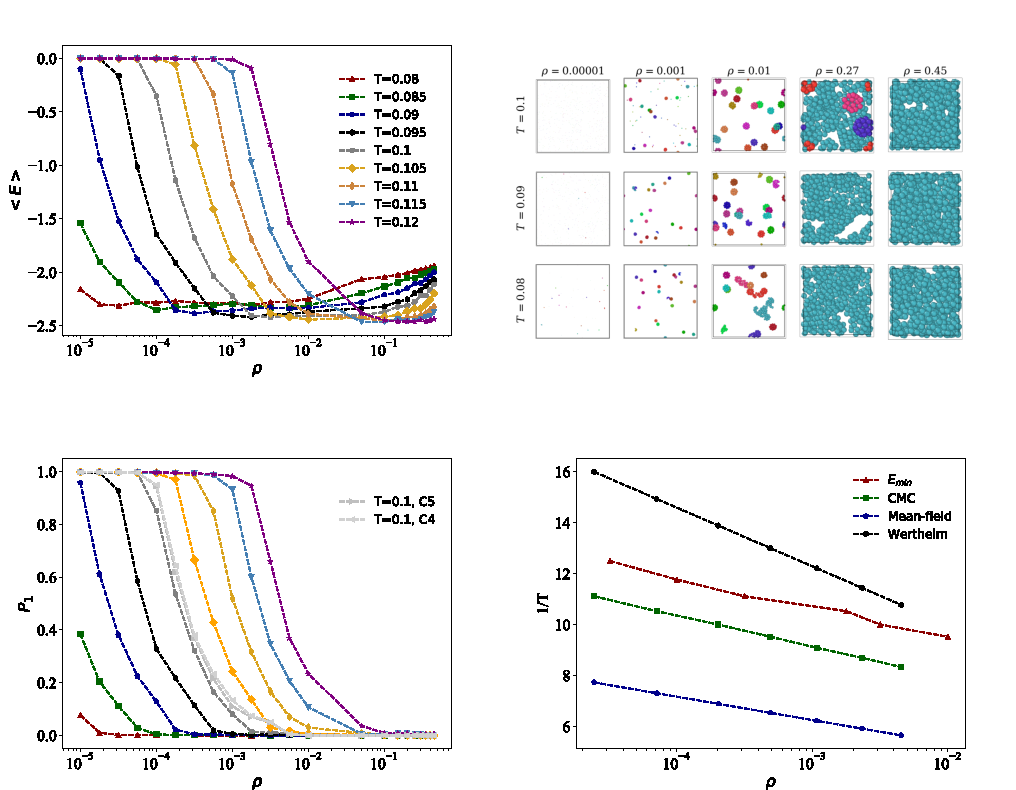
\includegraphics{fig5.pdf}
	\caption{\label{Energy} a) Average potential energy per particle as a function of density for different isotherms. For clarity, the x-axis is in log-scale. We observe a non-monotonic behaviour of the average energy characteristic of self-assembly systems. b) Frontal snapshots of the system for different densities and temperatures. Images were obtained with OVITO, where the colors represent particles that belong to the same cluster. For low densities, some colors repeat themselves even though particles are not bounded due to the large number of unbounded particles which count as clusters of size one. c) Fraction of monomers as a function of the density. Two new curves were added at $T=0.1$, with a different solution (as shown in Fig.~\ref{Yield}). d) Inverse temperature as a function of density for the point at which the fraction of monomers is equal to $50\%$ (critical micelle concentration). A theoretical curve is drawn to estimate the CMC, it is calculated using Eq.~\eqref{meanfield}. The curve corresponding to the energy minimum in a) is also shown. All results were simulated with the one specie and two color design (except for the two curves in the top right plot), with $\gamma=90^\circ$ and a $\cos\theta_{max}=0.98$.}
\end{figure*}

In Fig.~\ref{Energy} we present a study of the phase behavior of the two color solution, C2(1). For simplicity, we restrict ourselves to the parameters $\cos\theta_{max}=0.98$ and $\gamma=90^\circ$, a combination which favors the snub cube structure. In panel \emph{a} we plot the Energy-vs-density, $E(\rho)$, curve at different temperatures, where we observe a non-monotonic behavior of the average energy $E(\rho)$ with increasing density. This behaviour is characteristic of the self-assembly of finite-size aggregates~\cite{Sciortino2009}: at low densities the system is in a gas phase of mostly monomers (unbounded particles); with increasing density particles start to aggregate and the energy decreases approaching the value $E=5/2$ (in units of $\epsilon$) which corresponds to an ideal gas phase of fully formed aggregates; for larger densities the gas phase competes with a percolated liquid phase that, due to geometric constraints originating from the patches arrangement on the surface of the particle, cannot form all available bonds and has thus higher energy than the gas phase. A thermodynamic motivation for the link between a $E(\rho)$ minimum and phase separation is discussed in Ref.~\cite{Russo2021}. Fig.~\ref{Energy}b shows shapshots of Monte Carlo simulations of increasing densities and at three different temperatures, displaying the transition between a gas of monomers, to a gas of snub cubes, to a percolated liquid phase.



%Here, the density is large enough and the temperature low enough for particles to bound and remain bounded until a snub cube is formed. These shells are the equilibrium structures for the patchy particles used. Since the density is still quite low, the average distance between clusters will be large enough such that they will rarely interact with each other over the course of the simulations, which leads to the gas of clusters.
%For large densities, the liquid phase is approached and less clusters are formed leading to an increase of the average energy. Eventually the liquid phase percolates the system. These results in combination with the snapshots shown suggest there is a possible phase separation of the liquid and gas phase. Future studies should focus on the characterization of the phase space of these structures.

In Fig.~\ref{Energy}c we plot the fraction of monomers as a functions of density for the same state points as above, and additionally for the designs C4(1) and C5 at $T=0.1$.
%We find that the behavior for lower densities is similar independently of the design used; it becomes relevant only at higher densities. This suggests that mean field theories, like Wertheim theory \cite{Chapman1989}, might be able to describe these systems at low densities independently of design used.
From this, we measure the critical micelle concentration (CMC), defined as the number density at $50\%$ of particles are in a monomeric state ($\rho_1=0.5$). The CMC is plotted with (green) squares in Fig.~\ref{Energy}d, where it is seen to have an exponential behaviour as a function of the inverse temperature, $1/T$. We also plot the points corresponding to the minima of the energy, which also show a similar exponential increase. The slope of these curves is well captured by 
the mean-field prediction (blue symbols)~\cite{Kraft2012}
%, where assumes that the entropy loss is purely translational (see Ref.~\cite{Kraft2012} for a derivation) and predicts an exponential decay of the density of monomers

\begin{equation}\label{meanfield}
\rho_1=\frac{1}{V_b}\exp[\frac{c(n)}{(n-1)} \frac{\varepsilon}{k_B T}]
\end{equation}



\noindent where $V_b$ is the bonding volume for the Kern-Frankel interaction and $c(n)/(n-1)$ is the average number of bonds per particle in the clusters. Using $c(n)/(n-1)$ as a fitting parameter~\cite{Hatch2016}, we employ a least-squares minimization to fit the simulation results for the CMC. We find a value of $c(n)/(n-1)\approx 1.728\pm 0.006$ best approximates the line shown in Fig.~\ref{Energy}.

%For our Monte Carlo simulations the value estimated is $c(n)/(n-1)\approx 2.51$, which is used for the line in Fig.~\ref{Energy}.

%The second prediction for $\rho_1$ is estimated using Wertheim theory \cite{Sciortino2007, Russo2021}:

%\begin{equation}\label{wertheim}
%\rho_1 = \rho X_1 X_2 X_3 X_4 X_5
%\end{equation}

%\noindent where $X_\alpha$ is the probability that patch $\alpha\in\left[1,\cdots, 5\right]$ is non-bounded, and computed through Eq.~\ref{prob}. It can be proven that the mean-field and Wertheim predictions coincide in the limit of high-temperatures~\cite{Russo2021}.

% Put in the appendix

%With the design used, the three top patches have the same colour which is different from the bottom two patches, as such, the relevant equations are:

%\begin{equation}
%X_1+X_2+X_3=\frac{3}{1+\rho \Delta (X_1+X_2+X_3)}
%\end{equation}

%\begin{equation}
%X_4+X_5=\frac{2}{1+\rho \Delta (X_4+X_5)}
%\end{equation}

%The strength of the interactions between interacting patches, $\Delta$, is given by:

%\begin{equation}\label{delta}
%\begin{split}
%\Delta & = \frac{V_b (e^{\beta\varepsilon}-1)}{(1-\phi)^3} \bigg[ 1 - \frac{5}{2} \frac{(3\sigma^2+8\delta\sigma+3\delta^2)}{\sigma(15\sigma+4\delta)}\phi \\
%& - \frac{3}{2}\frac{(12\delta\sigma+5\delta^2)}{\sigma(15\sigma+4\delta)}\phi^2 \bigg]
%\end{split}
%\end{equation}

%\noindent where $\phi=\pi\rho\sigma^3/6$ is the volume fraction and $\beta=1/k_B T$.


%The theory deviates slightly from the simulation, with the mean-field model getting closer results. This might be due to taking the average bonds per particle explicitly in the formula which is taken directly from the simulations. On the other hand, Wertheim theory does not require any previous measurement. It also does not take into account the specific orientation of the patches, which in our case is quite anisotropic, given that all patches are only on one half of the particle. This biases assembly to the specific structures discussed previously, while making others improbable (for example chains).

\end{document}


